
%(BEGIN_QUESTION)
% Copyright 2006, Tony R. Kuphaldt, released under the Creative Commons Attribution License (v 1.0)
% This means you may do almost anything with this work of mine, so long as you give me proper credit

A tank expert system gives the following pressure indications from its three transmitters:

$$\includegraphics[width=15.5cm]{i00256x01.eps}$$

From these pressure measurements, determine the level of liquid in the vessel and its specific gravity.  Also, write mathematical equations for calculating both these parameters given the three pressure sensor measurements.

\underbar{file i00256}
%(END_QUESTION)





%(BEGIN_ANSWER)

The ``Top'' transmitter's measurement of 50 inches water column tells us that the vessel is pressurized.  This figure will be important to include in our level calculations later.

The difference between ``Bottom'' and ``Middle'' pressure transmitter measurements is solely a function of liquid density, since the vertical distance between the two transmitters is fixed and any vapor pressure buildup (50 "W.C., as indicated by the ``Top'' transmitter) adds equally to {\it both} transmitters' indications.  In this case, the difference between 310 inches water column and 220 inches water column is 90 inches of water column:

\vskip 10pt

(310 "W.C.) - (220 "W.C.) = 90 "W.C.

\vskip 10pt

If the process liquid were water (S.G. = 1), the pressure difference would be 120 inches of water column, not 90, because the two transmitters are located 10 feet apart from each other.  Thus, the density of this liquid is substantially less than that of water:

\vskip 10pt

Specific gravity = (90 "W.C. / 120 "W.C.) = 0.75

\vskip 10pt

To calculate liquid level (height), we must first subtract the measured vapor pressure (50 "W.C.) from the ``Bottom'' pressure transmitter's indication, so that we are left with the pressure due to liquid head alone:

\vskip 10pt

hydrostatic pressure = (310 "W.C.) - (50 "W.C.) = 260 "W.C. 

\vskip 10pt

Dividing this hydrostatic pressure by the specific gravity yields the liquid column height:

\vskip 10pt

(260 "W.C.)/(0.75 "W.C. / in) = 346.67 inches or 28.89 feet

\vskip 30pt

Equations for calculating specific gravity and liquid level (let $x$ be the distance between the middle and bottom pressure transmitters in units of inches, and all pressures in units of inches water column):

$$\hbox{Specific Gravity} = {{P_{bottom} - P_{middle}} \over x}$$

\vskip 10pt

$$\hbox{Liquid level} = {{P_{bottom} - P_{top}} \over \hbox{Specific Gravity}}$$

$$\hbox{Liquid level} = x{{P_{bottom} - P_{top}} \over {P_{bottom} - P_{middle}}}$$


%(END_ANSWER)





%(BEGIN_NOTES)

%INDEX% Measurement, level: hydrostatic pressure
%INDEX% Measurement, level: tank expert system

%(END_NOTES)


